\documentclass[12pt,a4paper]{article}
\usepackage[warn]{mathtext}
\usepackage[utf8]{inputenc}
\usepackage[T2A]{fontenc}
\usepackage[english,russian]{babel}
\usepackage{indentfirst}
\usepackage{misccorr}
\usepackage{subcaption}
\captionsetup{compatibility=false}
\usepackage{graphicx}
\usepackage{wrapfig}
\usepackage{amsmath}
\usepackage{floatflt}
\usepackage{float}
\usepackage{amssymb}
\usepackage{color}
\usepackage{lscape}
\usepackage{hvfloat}
\usepackage{amsfonts}
\usepackage{euscript}


\graphicspath{ {images/} }
\usepackage{multicol}
\setlength{\columnsep}{2cm}


\begin{document}

\begin{titlepage}
	\centering
	\vspace{5cm}
	{\scshape\LARGE Московский физико-технический институт \par}
	\vspace{5cm}

	{\huge Лабораторная работа № 3.4.2 \par}
	\vspace{1cm}
	{\scshape\Large "Закон Кюри-Вейсса"\par}
	\vspace{2cm}
	\vfill
\begin{flushright}
	{\Large Выполнила студентка Б04-906}\par
	\vspace{0.3cm}
	{\LARGE Прохорова Юлия} \par

	
\end{flushright}
	

	\vfill\large

% Bottom of the page
	Долгопрудный, 2020 г.
\end{titlepage}

\section{Цель работы:}
Изучение температурной зависимости магнитной восприимчивости ферромагнетика выше точки Кюри.

\section{Оборудование:}
Катушка самоиндукции с образцом из гадолиния термостат, частотомер, цифровой вольтметр, LC-автогенератор, термопара медь-константан.

\section{Теоретическая часть}
% \textbf{Изучение магнитной индукции в образцах.} Магнитную индукцию удобно определять с помощью ЭДС, возникающей при изменении магнитного 
% потока $\text{Ф}$ в катушке, намотанной на обрзец:

% \begin{equation}
%     \varepsilon = -\frac{dФ}{dt}, \label{eq:ref}
% \end{equation}
Вещества с отличными от нуля атомными магнитными моментами обладают парамагнитными свойствами. Внешнее магнитное поле ориентирует магнитные моменты, 
торые в отсутствие поля располагались в пространстве хаотичным образом. 
\hyphenation{}
При повышении температуры $T$ возрастает дезориентирующее действие теплового движения частиц, и магнитная восприимчивость парамагнетиков убывает, 
в простейшем случае (в постоянном магнитном поле) по закону Кюри:

\begin{equation}
    \chi = \frac{C}{T}, \label{eq:re}
\end{equation}
где $C$ - постоянная Кюри. 
\hyphenation{}
Для парамагнитных веществ, которые при понижениитемпературы становятся ферромагнитными, формула \eqref{eq:re}  должна быть видоизменена.
Эта формула показывает, что температура $T=0$ является особой точной температурной кривой, в которой $\chi$ неограниченно возрастает.
При $T \rightarrow 0$  тепловое движение всеменьше препятствует магнитным моментам атомов ориентироваться в одном направлении при сколь угодно слабом
 внешнем поле. В ферромагнетиках - под влиянием обменных сил - это происходит при понижении температуры до неабсолюного нуля, а до температу ры Кюри  $\Theta$.

\begin{figure}[H]
    \begin{center}
    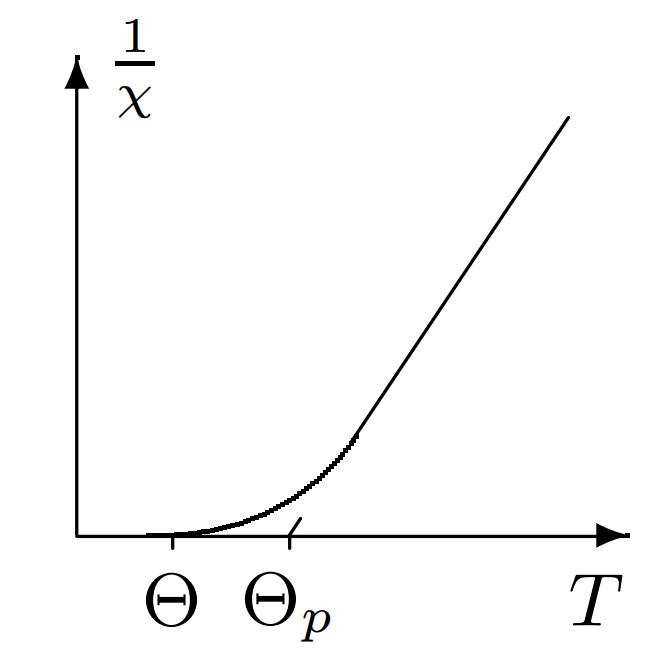
\includegraphics[width=6cm]{зависимость_в_точке_Кюри.png}
    \caption{Зависимость обратной величины магнитной восприимчивости от температуры}
    \label{kuri} %% метка рисунка для ссылки на него
    \end{center}
\end{figure}

Оказывается, что у ферромагнетиков закон Кюри заменияется законом Кюри-Вейсса:

\begin{equation}
    \chi \sim \frac{1}{T-\Theta_p}, \label{eq:f_kuri_veis}
\end{equation}
где $\Theta_p$ - температура близкая к температуре Кюри. 
\hyphenation{}
    Эта формула хорошо описывает поведение ферромагнитных веществ после их перехода в парамагнитную фазу при заметном удалении температуры от $\Theta$, но недостаточно точна при $T\approx \Theta$.
\hyphenation{}
Иногда для уточнения формулы \ref{eq:f_kuri_veis} вводят вместо одной две температуры Кюри,  одна из которых описывает точку фазового перехода - ферромагнитная точка Кюри $\Theta$, а другая является параметром в формуле 
\ref{eq:f_kuri_veis} - парамагнитная точка Кюри - $\Theta_p$ (рис.\ref{kuri}).

\section{Экспериментальная установка}
Схема установки для проверки Кюри-Вейсса изображена на рис. \ref{scheme}. Исследуемый ферромагнитный образец (гадолиний) расположен внутри пустотелой катушки самоиндукции, которая служит индуктивностью
 колебательного контура, входящего в состав $LC$-автогенератора. Автогенератор собран на полевом транзисторе КП-103 и смонтированв виде отдельного блока.

\begin{figure}[H]
    \begin{center}
    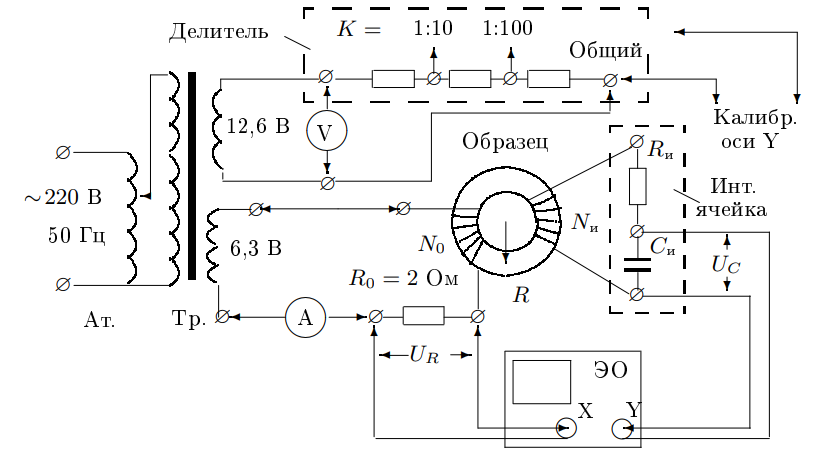
\includegraphics[width=10cm]{scheme.png}
    \caption{Схема экспериментальной установки}
    \label{scheme} %% метка рисунка для ссылки на него
    \end{center}
\end{figure}

Гадолиний является хорошим проводником электрического тока, а рабочая частота генератора достаточно велика ($\sim50 кГц$), поэтому для уменьшения вихревых токов образец изготовлен из мелких кусочков размером около 0,5 мм.
 Катушка 1 с образцом помещена в стеклянный сосуд 2, залитый трансформаторным маслом. Масло предохранняет образец от окисления и способствует ухудшению электрического контакта между отдельными частичками образца. Также он
  улучшает тепловой контакт контакт между образцом и термостатируемой (рабочей) жидкостью 3 в термостате. Ртутный термометр 4 используется для приближенной оценки температуры. Температура образца регулируется с помощью термостата.
\hyphenation{}
Магнитная восприимчивость образца $\chi$ определяется по изменению самоиндукции катушки собразцом и через $L_0$ -её самоиндукцию в отсутствие образца, получим:

\begin{equation}
    (L-L_0) \sim \chi, \label{eq:L}
\end{equation}
При изменении самоиндукции образца меняется период колебаний автогенератора: 

\begin{equation}
    \tau = 2\pi\sqrt{LC}, \label{eq:L}
\end{equation}
где $C$ - ёмкость контура автогенератора.
\hyphenation{} Период колебаний в отсутствие образца определяется самоиндукцией пустой катушки:
\begin{equation}
    \tau_0 = 2\pi\sqrt{L_0C}, \label{eq:tau}
\end{equation}

Из (\ref{eq:L}) и (\ref{eq:tau}) имеем:

\begin{equation}
    (L-L_0) \sim (\tau^2-\tau_0^2). \label{eq:tautau}
\end{equation}
Таким образом, 
\begin{equation}
    \chi \sim (\tau^2-\tau_0^2). \label{eq:itog}
\end{equation}

Из формул (\ref{eq:f_kuri_veis}) и (\ref{eq:itog}) следует, что закон Кюри-Вейсса справедлив, если
выполнено соотношение
\begin{equation}
    \frac{1}{\chi} \sim (T - \Theta_p) \sim \frac{1}{(\tau^2-\tau_0^2)}. \label{eq:main}
\end{equation}
Для охлаждения образца используется холодная водопроводная вода, циркулирующая вокруг сосуда с рабочей жидкостью(дистиллированной водой) : рабочая жидкость постоянно перемешивается.
\hyphenation{} Величина стабилизируемой температуры задается на дисплее 5 термостата. При примближении к заданной температуре, непрерывный режим работы нагревателя автоматически переходит
в импульсный - процесс стабилизации температуры.
\hyphenation{}  При этом температура исследуемого образца несколько отличается от рабочей жидкости. Псоде того как вода достигла нужной темпертуры, идет медленный процесс выравнивания температур образца и воды.
Разность их температур контролируется с помощью медно-константановой термопары 6 и цифрового вольтметра. Один из контактов термопары находится в тепловом контакте с образцом, а другой погружен в воду.  

\section{Ход работы}

\begin{enumerate}
    \item Оценим допустимую ЭДС термопары, учитывая что постаянная темопары $k = 24 град/мВ$, а допустимая разница температур $\Delta T = 0,5  ^\circ C$ \\
$\varepsilon = 0,02 мВ$. 
    \item  Снимаем зависимость периода колебаний LC-генератора оттемпературы образца, отмечая
период колебаний $\tau $ по частотомеру, а температуру T -  по показаниям дисплея и цифровому вольтметру.

\begin{table}[H]
    \centering
    \begin{center}
    \end{center}
    \vspace{0.1cm}
    \label{tab:my_label}
    \begin{tabular}{ |p{2cm}|p{2cm}|p{2cm}|p{2cm}|}
 \hline
 № & $T  ^\circ C$ & $\tau, мкс$ & $1/(\tau^2-\tau_0)$ \\
 \hline
    1 & 13.18 & 10.756 & 0.030 \\
 \hline
    2 & 14.41 & 10.676 & 0.031\\
   \hline
    3 & 17.64 & 10.565 & 0.034\\
    \hline
    4 & 19.67 & 10.329 & 0.040\\
 \hline
    5 & 21.66 & 9.996 & 0.055\\
   \hline
    6 & 23.69 & 9.607 & 0.095\\
    \hline
    7 & 25.62 & 9.442 & 0.136\\
 \hline
    8 & 27.62 & 9.349 & 0.179\\
   \hline
    9 & 29.57 & 9.289 & 0.224\\
    \hline
    10 & 31.66 & 9.257 & 0.258\\
 \hline
    11 & 33.64 & 9.231 & 0.294\\
   \hline
    12 & 35.63 & 9.210 & 0.332\\
    \hline
    13 & 37.62 & 9.195 & 0.365\\
 \hline
    14 & 39.63 & 9.182 & 0.400\\
\hline
\end{tabular}
\caption{Получение данных}
\end{table}
\item Построим график зависимости $\frac{1}{\tau^2-\tau_0^2}= f(T)$. Экстраполируя полученную прямую к оси абсцисс, определяем парамагнитную точку Кюри $\Theta_p$ для гадолиния.

\begin{figure}[H]
    \begin{center}
    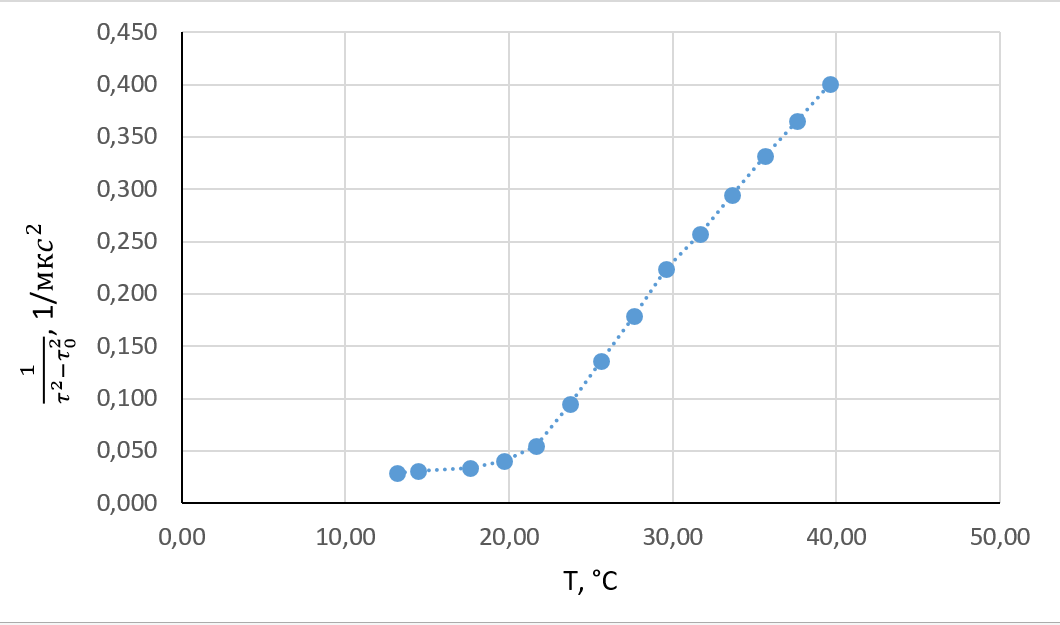
\includegraphics[width=10cm]{график_1.png}
    \caption{График зависимость f(T)}
    \label{ferrit} %% метка рисунка для ссылки на него
    \end{center}
\end{figure}

\begin{figure}[H]
    \begin{center}
    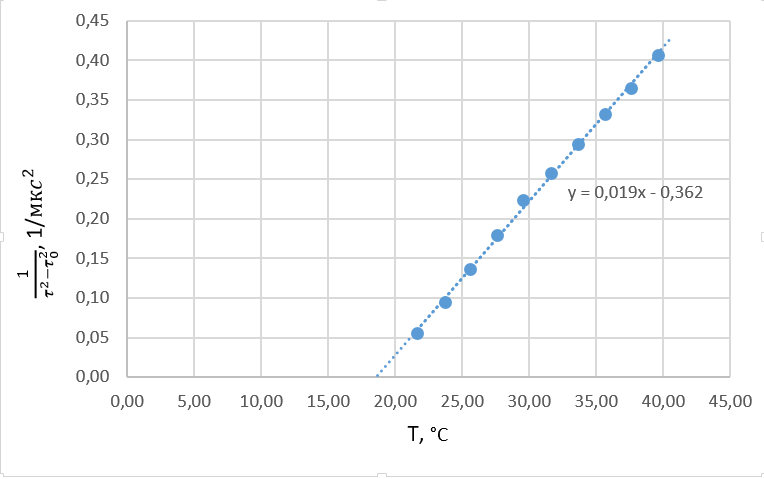
\includegraphics[width=10cm]{график_2.png}
    \caption{Экстраполяция полученной линейной зависимости}
    \label{pe} %% метка рисунка для ссылки на него
    \end{center}
\end{figure}
    
\end{enumerate}
Плучили $\Theta_p = 18.9 \pm 0.9 ^\circ C$. 
Табличное значение: $\Theta_p = 20.2 ^\circ C$
\section{Вывод}

В ходе лабораторной работы:
\begin{enumerate}
    \item Изучили температурную зависимость магнитной восприимчивостью гадолиния выше точки Кюри.
    \item Рассчитали значение температуры в точке Кюри $\Theta_p = 18.9$. Относительная огрешность составила $\varepsilon =  6\%$.
\end{enumerate}
\newpage
\end{document}